\documentclass{beamer}
\usepackage{graphicx}
\graphicspath{{img/}}
\usepackage{ragged2e}
\usepackage{amsmath}

\usetheme{singapore}
\begin{document}

\begin{frame}
    \centering
    
\includegraphics[height=0.2\textheight]{img/moogle.png}
    Primer proyecto de programaci\'on I\\\small Karla D\'iaz Saura C113
\end{frame}
%------------------------------------------------------------------------
\section*{Qu\'e es Moogle!}
\begin{frame}
    \frametitle{\textbf{>Qu\'e es Moogle?}}
    \begin{itemize}
        \item Sistema básico de recuperaci\'on de la informaci\'on.\pause
        \item Permite encontrar informaci\'on dentro de grandes colecciones de documentos a trav\'es de b\'usquedas utilizando palabras clave.\pause
        \item Posee opciones de b\'usqueda avanzada para aumentar la precisi\'on de los resultados obtenidos seg\'un la necesidad del usuario.\pause
        \item Se basa en el modelo vectorial de recuperaci\'on de informaci\'on.
    \end{itemize}
\end{frame}
%------------------------------------------------------------------------
\section{Modelo vectorial}
\begin{frame}
    \frametitle{\textbf{Modelo vectorial\\de recuperaci\'on de la informaci\'on}}
    \begin{itemize}
        \item Consiste en la representaci\'on de documentos y consultas como vectores en un espacio multidimensional.
        \item Usa la similitud de coseno para determinar la relevancia de un documento respecto a la consulta.
    \end{itemize}
    \vspace{1cm}
    \hspace*{5cm}
    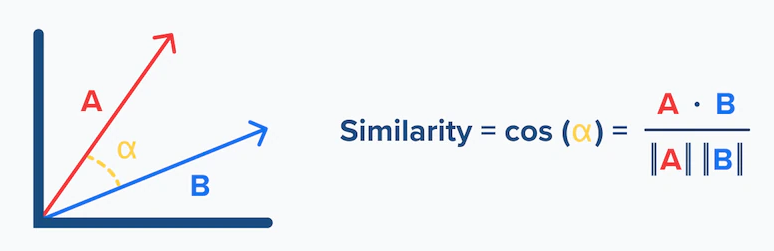
\includegraphics[width=0.5\textwidth,height=0.2\textheight]{./img/simcoschulin.png}
\end{frame}
%------------------------------------------------------------------------
\begin{frame}
    \frametitle{Similitud del coseno}
    \begin{itemize}
        \item Mide la similitud sem\'antica entre dos vectores.\pause
        \item Se calcula como el coseno del \'angulo entre dos vectores (en este caso, un vector de consulta y su correspondiente vector de documento)\pause
        \item Un valor de similitud del coseno de 1 indica que los dos vectores son id\'enticos, mientras que un valor de 0 indica que los vectores son completamente diferentes.
    \end{itemize}
\end{frame}
%------------------------------------------------------------------------
\begin{frame}
    \frametitle{Similitud del coseno}
    \framesubtitle{Representaci\'on gr\'afica}
    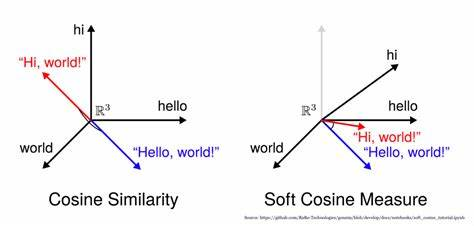
\includegraphics[width=\textwidth]{./img/simcos.jpg}
\end{frame}
%------------------------------------------------------------------------
\section{Etapas de Moogle!}
\begin{frame}
    \frametitle{\textbf{Tres etapas\\en el funcionamiento de Moogle!}}
    \begin{enumerate}
        \item Creaci\'on de la base de datos.
        \item Procesamiento de la consulta.
        \item C\'alculo de resultados.
    \end{enumerate}
    
\end{frame}
%------------------------------------------------------------------------
\begin{frame}
    \frametitle{Creaci\'on de la base de datos}
    \framesubtitle{Preprocesamiento de la informaci\'on}
    Al ejecutar el programa, se leen todos los documentos del directorio \textit{Content} y se almacena la informaci\'on en tres estructuras:
    \vspace{0.2cm}
    \begin{itemize}
        \item  \small Diccionario \textbf{$<$string, string[ ]$>$ TituloTexto},que almacena el t\'itulo de cada documento y su texto correspondiente.
        \item \small Diccionario \textbf{$<$int, string$>$ docID\_Title},que almacena cada documento en funci\'on de un identificador.
        \item Diccionario \textbf{$<$string, Dictionary$<$int, double$>>$ Vocabulary}
        que, junto al vector de consulta, constituyte la estructura central del an\'alisis
        de la informaci\'on.
    \end{itemize}
\end{frame}
%------------------------------------------------------------------------
\begin{frame}
    \frametitle{Creaci\'on de la base de datos}
    \framesubtitle{Vocabulario como estructura de optimizaci\'on de la b\'usqueda}
    \begin{columns}
        \begin{column}{0.5\textwidth}
            \centering
            \justifying
            El diccionario \textbf{Vocabulary} almacena como claves todos los t\'erminos que aparecen al menos una vez en alguno de los documentos, y como valores diccionarios donde se encuentran los \textbf{ID} de los documentos que contienen el t\'ermino y el valor de \textbf{TF} de este en cada documento. 
        \end{column}
        \begin{column}{0.5\textwidth}
            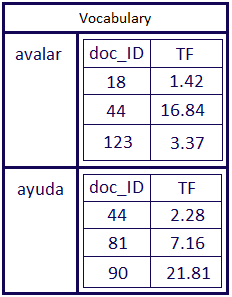
\includegraphics[height=0.7\textheight,width=\textwidth]{./img/vocab.png}
        \end{column}
    \end{columns}
\end{frame}
%------------------------------------------------------------------------
\begin{frame}
    \frametitle{Creaci\'on de la base de datos}
    \framesubtitle{Vocabulario como estructura de optimizaci\'on de la b\'usqueda}
    \centering
    >Por qu\'e es eficiente esta forma de almacenar la informaci\'on?
\end{frame}
%------------------------------------------------------------------------
\begin{frame}
    \frametitle{Procesamiento de la consulta}
    La b\'usqueda se realiza a partir de la consulta introducida por el usuario. Como existe la opci\'on de b\'usqueda avanzada, el usuario puede marcar alguno de los t\'erminos de su consulta con un \textbf{operador}, marcando as\'i la prioridad que concede este.
    
\end{frame}
%------------------------------------------------------------------------
\begin{frame}
    \frametitle{Procesamiento de la consulta}
    \framesubtitle{Operadores de la b\'usqueda avanzada}
    \textbf{Moogle!} cuenta con dos operadores:
    \vspace*{3mm}
    \begin{itemize}
        \item Operador de no aparición \textbf{(!)}:
        
        \vspace*{0.8mm}
        \small\textit{Ejemplo de uso: “!término”}

        \small La presencia de este operador al inicio de una palabra indicará que esta no deberá 	aparecer en ninguno de los documentos que se devuelvan como resultado.
        \vspace{3mm}
        \item Operador de aparición requerida \textbf{(\textasciicircum)}:
        
        \vspace*{0.8mm}
        \small\textit{Ejemplo de uso: “\textasciicircum término”}

        La presencia de este operador al inicio de una palabra indicará que esta deberá aparecer en todos los documentos que se devuelvan como resultado.
    \end{itemize}
\end{frame}
%------------------------------------------------------------------------
\begin{frame}
    \frametitle{Procesamiento de la consulta}
    \framesubtitle{Transformando cadenas en vectores}
    La estructura \textit{"vector"} consiste en un diccionario \textbf{$<$string, double$>$} que almacena como claves a los t\'erminos de la consulta y como valores al peso (expresado en \textit{TF*IDF}) de cada t\'ermino.
    \vspace{5mm}
    Un vector puede tener como m\'aximo un n\'umero de \textit{"componentes"} igual al n\'umero de t\'erminos de la consulta. Asimismo, puede haber vectores compuestos por menos t\'erminos que los de la consulta.
\end{frame}
%------------------------------------------------------------------------
\begin{frame}
    \frametitle{Procesamiento de la consulta}
    \framesubtitle{Vectores de consulta}
    Dada la posibilidad de modificar la relevancia de los t\'erminos de la consulta usando operadores, es necesario tener en cuenta tres tipos de vectores de consulta:
    \vspace{1mm}
    \begin{itemize}
        \item Vectores \textbf{OR}:
        
        \small Contienen todos los términos de la consulta, se encuentren o no marcados con un operador.
        \vspace{1mm}
        \item Vectores \textbf{NOT}:
        
        \small Contienen términos marcados con el operador “\textbf{!}”.
        \vspace{1mm}
        \item Vectores \textbf{MUST}:
        
        \small Contienen términos marcados con el operador “\textbf{!}”.
    \end{itemize}
\end{frame}
%------------------------------------------------------------------------
\begin{frame}
    \frametitle{Procesamiento de la consulta}
    \framesubtitle{Vectores de consulta}
    \centering 
    >Cu\'antos vectores de consulta se crean para una b\'usqueda?
    \vspace{5mm}
    \justifying
    \begin{itemize}
        \item Un solo vector \textbf{OR} con todos los t\'erminos de la consulta.
        \vspace{1mm}
        \item Tantos vectores \textbf{NOT} como t\'erminos haya marcados en la consulta.
        \vspace{1mm}
        \item Tantos vectores \textbf{MUST} como t\'erminos haya marcados en la consulta.
    \end{itemize}
    \vspace{1.6cm}
    %el \thanks{} no funciona en las presentaciones aparentemente
    \tiny *N\'otese que tanto los vectores NOT como los MUST tendr\'an cada uno una sola componente
\end{frame}
%------------------------------------------------------------------------
\begin{frame}
    \frametitle{Procesamiento de la consulta}
    \framesubtitle{Vectores de consulta}
    Habiendo obtenido un n\'umero variable de vectores, >c\'omo se puede determinar qu\'e documento es m\'as relevante para el usuario? \pause
    \vspace{5mm}
    
    Para obtener el vector final que se utilizar\'a en el c\'alculo de la similitud del coseno, se opera el vector \textbf{OR} con:
    \begin{enumerate}
        \item Los vectores \textbf{MUST}
        
        \small Se elimina del vector de \textbf{OR} todo documento que no coincida con el resultado de todos los vectores \textbf{MUST}.
        
        \item Los vectores \textbf{NOT}
        
        Se elimina del vector de \textbf{OR} todo documento que coincida con el resultado de al menos uno de los vectores \textbf{NOT}.
        

    \end{enumerate}

\end{frame}
%------------------------------------------------------------------------
\begin{frame}
    \frametitle{Procesamiento de la consulta}
    \framesubtitle{Vectores de documento}
    Para calcular la similitud del coseno necesitamos comparar el vector de consulta con los vectores de cada documento seg\'un la consulta. Estos ser\'an creados de la misma forma que se crea el vector \textbf{OR} de consulta.
\end{frame}
%------------------------------------------------------------------------
\begin{frame}
    \frametitle{C\'alculo de resultados}
    \framesubtitle{Similitud del coseno}
    \justifying
    La similitud del coseno se calcula como la raz\'on entre el producto escalar de ambos vectores entre el producto de sus normas.
    \vspace{1.5mm}

    \centering
    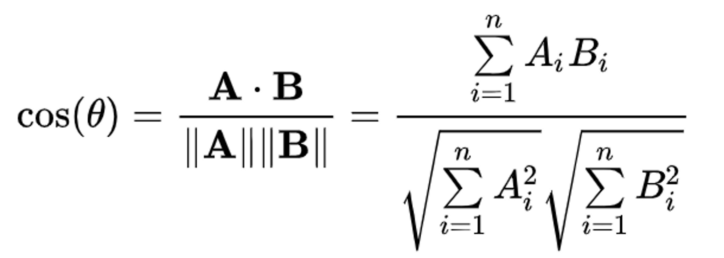
\includegraphics[width=0.7\textwidth]{./img/formula.png}
    \vspace{1.5mm}

    \justifying
    \textbf{Moogle!} crea el vector final de consulta y los vectores de documentos con componentes cuyos valores ya son $x=\frac{A}{||A||}$. Por tanto, el score de cada documento se obtiene simplemente calculando el producto escalar del vector de consulta y el vector de documento.
\end{frame}
%------------------------------------------------------------------------
\section{Devoluci\'on de resultados}
\begin{frame}
    \frametitle{\textbf{Devoluci\'on de resultados}}
    Los documentos que resultaron ser relevantes para el usuario se devuelven ordenados seg\'un su score. En la interfaz de b\'usqueda, el usuario podr\'a conocer cu\'antos documentos coinciden con su b\'usqueda, cu\'ales son esos documentos en orden de relevancia y, por cada documento enla respuesta, recibir\'a la l\'inea del texto que contenga la mayor cantidad de palabras relevantes en su b\'usqueda.
\end{frame}

\end{document}